Der Weg bis \TOWN{Santa Barbara}, unserem ursprünglichen angedachten Ziel, gibt nichts her.
Danach ist man auch noch ein gutes Stück auf dem Freeway 101 unterwegs bevor es wirklich auf die \FOREIGN{Route~1} geht.
Ab dort verläuft sie dann auch sehr nah an der Küste entlang.
Hier und dort trifft man \FOREIGN{Vista Points}\footnote{Aussichtspunkte} an und bei dem mit den \FOREIGN{Elephant Seals} sind wir rausgefahren.
Am Strand lagen einige der Tiere herum, sonnten und nässten sich ein.
Letzteres muss dem Geruch nach zu urteilen mindestens drei bis vier Mal pro Tier passiert sein.

\newpage
\thispagestyle{empty}
\begin{tikzpicture}[remember picture, overlay]
\node[inner sep=0pt, yshift=-.25\paperheight] at (current page.north) {%
	\includegraphics[width=\paperwidth,height=.5\paperheight]{20/image20160419_164726302.jpg};%
};
%\node[inner sep=0pt, yshift=.25\paperheight] at (current page.south) {%
%	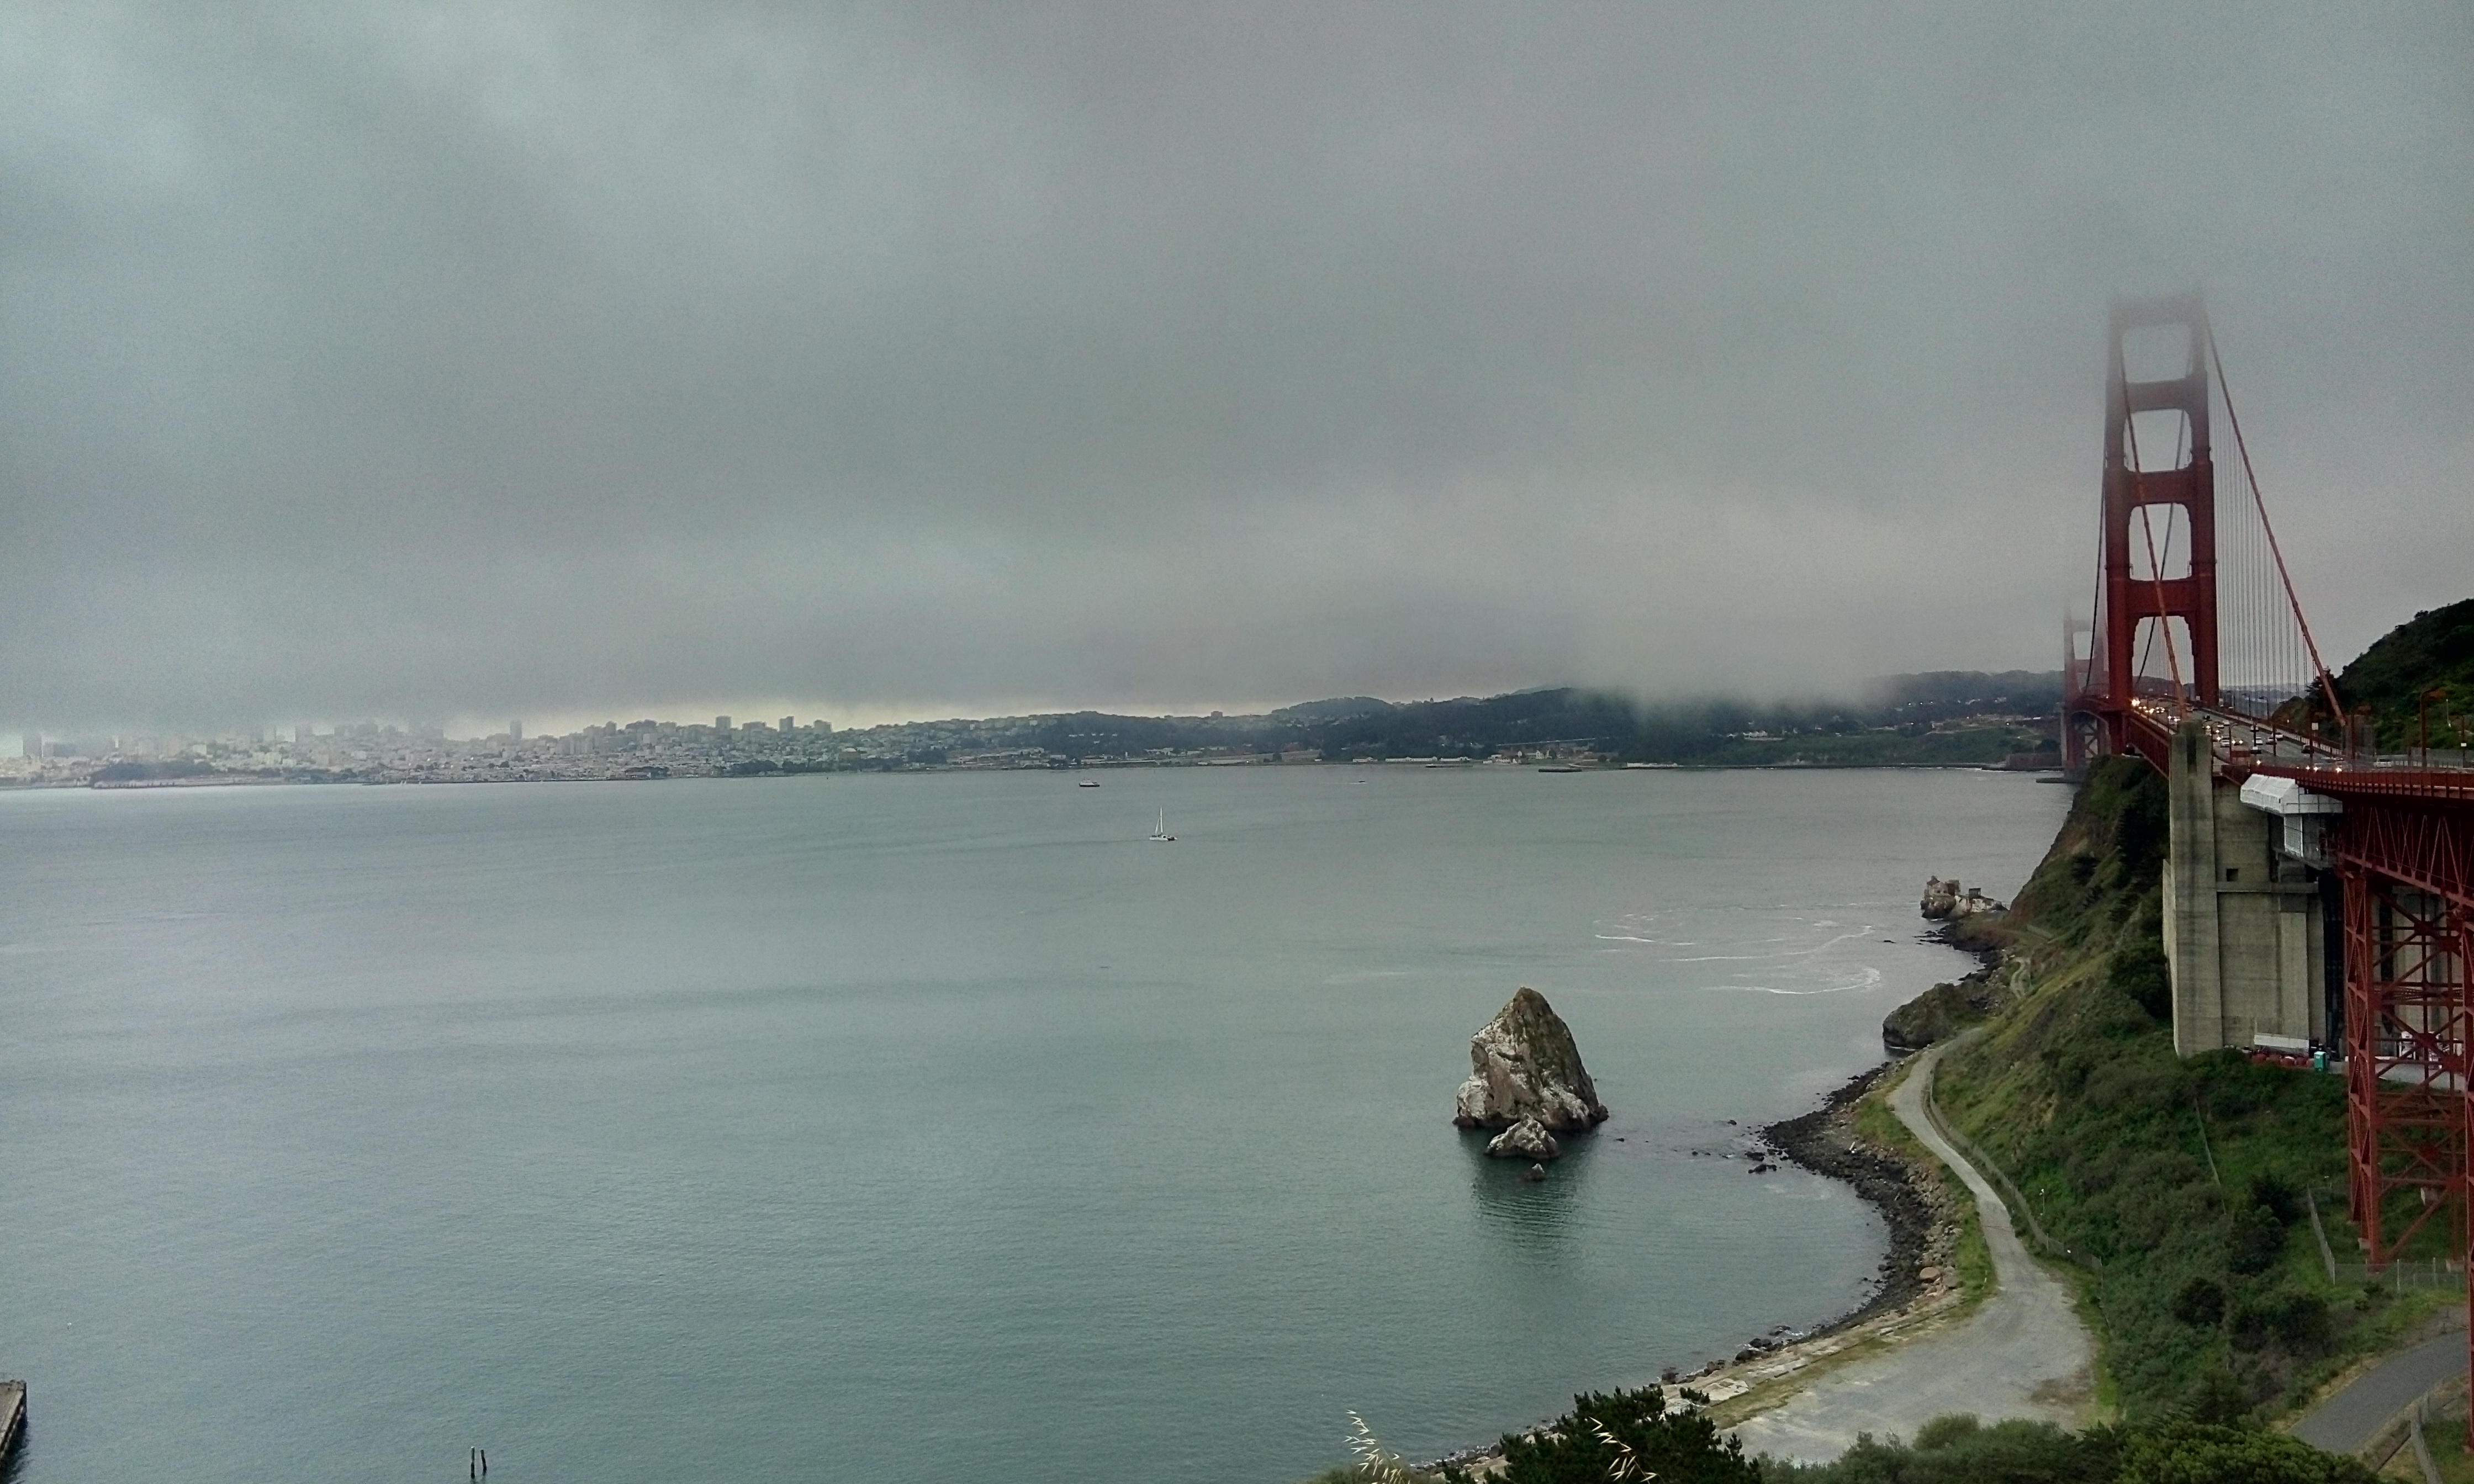
\includegraphics[width=\paperwidth,height=.5\paperheight]{21/image20160420_193101911.jpg};%
%};
\end{tikzpicture}
\newpage


Bis etwa hierhin war die Landschaft hügelig und nach einigen weiteren Meilen wurde die Küste richtig steil.
Die Straße schlängelte sich ab da so durch und die erlaubten 55~mph schafft man mit keinem Sportfahrwerk.
Zwischen 20 und 40~mph fährt man, wenn nicht beabsichtigt gute 100~m in die Tiefe zu \glqq fahren\grqq.

An einem Aussichtspunkt saßen zwei \FOREIGN{Hitchhiker}\footnote{Anhalter}, die ich eingepäckt hätte.
Vorausgesetzt wir wären in ihre Richtung gefahren, wobei ich mir gut vorstellen kann, dass die zwei überall hin mitgefahren wären, denn der Aussichtspunkt liegt mitten im Nirgendwo.
Der Christian hat die zwei jedoch gleich mal als Landstreicher diffamiert und sich quer gestellt.
Die nächsten Tramper gehen aber an Bord!

In Monterey geht es morgen ins Aquarium\dots wie spannend.
